% !TEX root = ../main.tex
% Evaluations
% Claims to support: VOTAG plateau and k-grid justification, leaderboard
% across approaches and model scales, bug-bias diagnosis, debiasing results.

\section{Evaluations}
\label{sec:evaluations}

% TODO

\subsection{RQ1. To what extent can similarity-weighted voting on the nearest neighbors classify issue reports, and at what point does adding neighbors stop helping?}
\label{sec:rq1}
\begin{figure}[t]
    \centering
    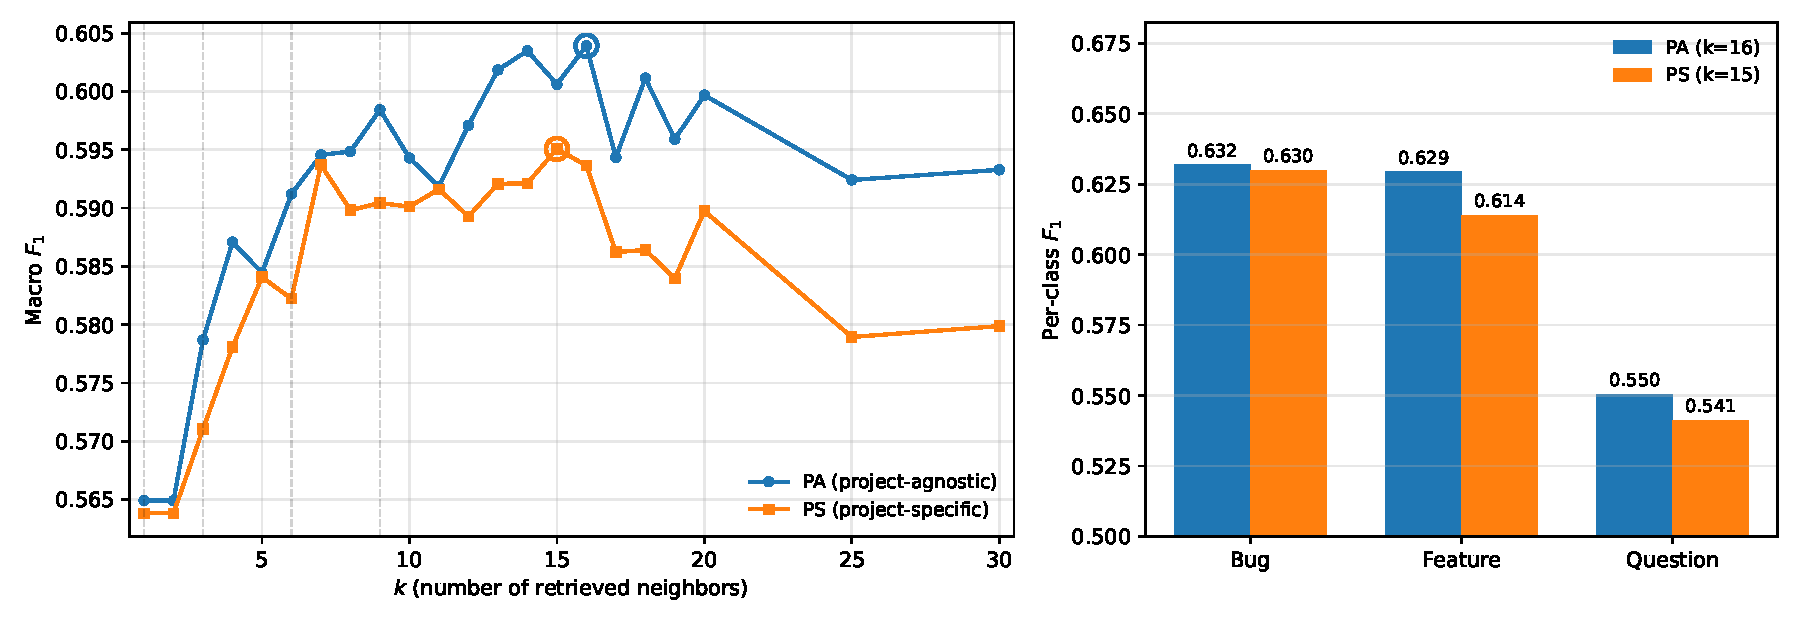
\includegraphics[width=\linewidth]{figures/vtag_kcurve.pdf}
    \caption{\textbf{(left)} \votag\ macro $F_1$ as a function of $k$ in both PS and PA settings. Circles mark peak performance. \textbf{(right)} Per-class $F_1$ at each setting's best $k$ ($k{=}15$ for PS, $k{=}16$ for PA).}
    \label{fig:vtag-kcurve}
\end{figure}

% TODO: motivate the k-sweep. Why scan k=1..30 instead of just one or two
% k values? Suggested points to cover:
%   (a) k is the only knob in VOTAG -- nothing else to tune, so the
%       sweep characterizes the entire design space.
%   (b) The plateau location empirically anchors the RAGTAG k grid in §3
%       (we use {0,1,3,6,9} because the curve flattens around k=7).
%   (c) Going up to k=30 lets us show diminishing returns and the decline
%       past the peak; a smaller range would hide the plateau.
% Insert as a 1--2 sentence framing right before "We evaluate ...".

We evaluate \votag's performance on both PA and PS settings at $k$ values 1 to 30. The resulting macro F1 scores are shown in \Cref{fig:vtag-kcurve}. \votag's best macro F1 is 0.595 ($k{=}15$) in PS and 0.604 ($k{=}16$) in PA. Both settings reach 99.8\% (PS) and 98.5\% (PA) of their respective peak by $k{=}7$. When adding neighbors beyond the peak, PS loses 0.015 and PA loses 0.011 by $k{=}30$.

PA consistently outperforms PS at every $k$. However, the performance gap is marginal: averaging 0.007 macro F1, with a maximum of 0.015 at $k{=}18$. This similar performance is due to the large overlap of the top-$k$ neighbors in both settings. Specifically, PA and PS share 84--90\% of the top-$k$ neighbors across $k\in[3,30]$. Therefore, even when using the full 3{,}300-issue retrieval index, most of the retrieved neighbors are from the same project. This means issue reports from the same project tend to be closer in the embedding space.

Question consistently has the weakest performance among the three labels at every $k$ in both settings. At best $k$, PS per-class F1 is 0.630 for bug, 0.614 for feature, and 0.541 for question. The corresponding PA values are 0.632, 0.629, and 0.550 (\Cref{fig:vtag-kcurve}). Additionally, questions are more frequently misclassified as bugs: 32\% of question issues are predicted as bugs in both settings, while 18\% (PS) and 17\% (PA) are predicted as features. Since \votag predicts the label with the most accumulated similarity weight, this misclassification asymmetry indicates that question issues are more similar to bugs than to features in the embedding space.

% TODO: write a transition sentence/paragraph closing RQ1 and leading into
% the next subsection. Suggested points to cover:
%   (a) Position VOTAG's ~0.60 macro F1 as the retrieval-only floor that
%       LLM-based methods (RAGTAG, Debiased RAGTAG, Fine-tune) must clear.
%   (b) Flag that the bug-bias / question-as-floor asymmetry observed here
%       is not unique to VOTAG -- it also shows up in the LLM-based
%       methods, motivating the bug-bias diagnosis subsection.
%   (c) Optional: name the specific RQ/subsection that picks up next.
%   (d) Note (relocated from §5.3): VOTAG's best (0.604) comes within 0.009
%       macro F1 of Qwen-3B zero-shot (0.613). A pure-retrieval heuristic
%       essentially matches the smallest LLM at zero-shot. Could go here
%       (descriptive form) or in §6 Discussion (interpretive form).


\subsection{RQ2. How well does retrieval-augmented few-shot prompting classify issue reports across model scales, and how does performance vary with the number of in-context examples?}
\label{sec:ragtag}

\begin{figure}[t]
    \centering
    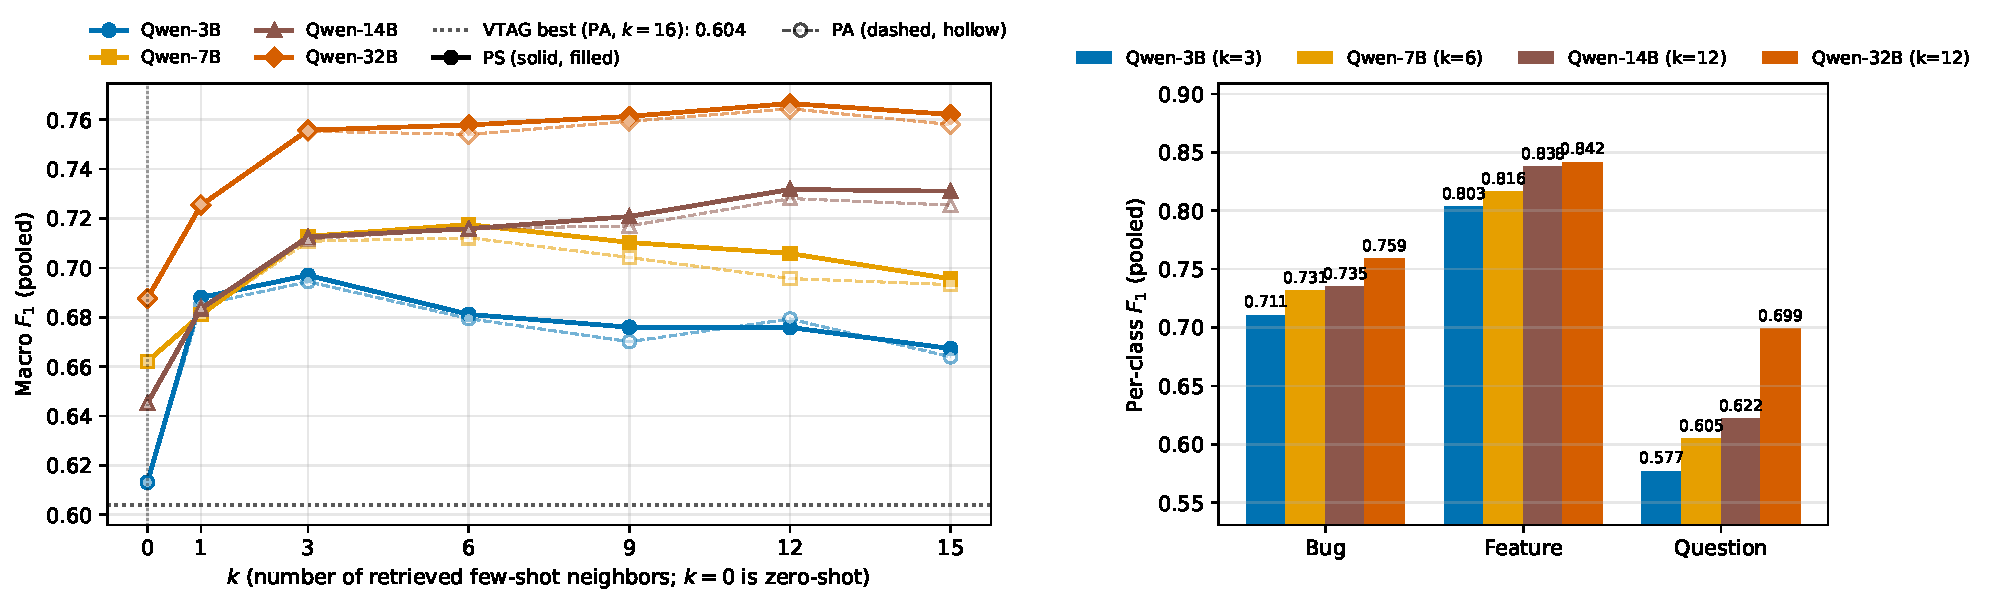
\includegraphics[width=\linewidth]{figures/ragtag_kcurve.pdf}
    \caption{\textbf{(left)} \ragtag\ macro $F_1$ as a function of $k$ for all four Qwen sizes. $k{=}0$ is the zero-shot baseline. The dotted horizontal line marks \votag's best (0.604, PA $k{=}16$). \textbf{(right)} Per-class $F_1$ for each model size at its best \ragtag-PS configuration.}
    \label{fig:ragtag-kcurve}
\end{figure}

We evaluate RAGTAG at $k$ values $\{0, 1, 3, 6, 9, 12, 15\}$ on both PA and PS settings, where $k{=}0$ is the zero-shot baseline~\cite{colavito2025benchmarking}. $k$ value grid selection is informed by \votag's peak performance around $k{=}15$ in the previous section. \Cref{fig:ragtag-kcurve} (left panel) shows the macro F1 of every model across this grid for both settings.

PS marginally outperforms PA at almost every (model, $k{\ge}1$) pair evaluated (zero-shot is identical between settings since no retrieval is performed). The close performance gap is due to the same top-$k$ neighbor overlap observed in the \votag analysis. The marginal improvement is significant because PS uses 11$\times$ less retrieval data per project: each PS index covers only its own 300 retrieval issues, while PA uses the full 3{,}300 across all 11 projects. Given this practical advantage, we conduct the rest of our RAGTAG analysis on the PS setting and report PS numbers throughout this section.

The best $k$ grows with model size: Qwen-3B peaks at $k{=}3$ (macro F1 = 0.697), Qwen-7B at $k{=}6$ (0.718), and both Qwen-14B and Qwen-32B at $k{=}12$ (0.732 and 0.767 respectively). This shows that larger models can use the context from additional examples more effectively. However, adding neighbors past $k{=}12$ has no benefit and slightly degrades performance: every model loses 0.001--0.015 macro F1 going from $k{=}12$ to $k{=}15$.

Every \ragtag\ configuration with $k{\ge}1$ outperforms the zero-shot baseline. At each model's peak, the gap over zero-shot averages +0.076 macro $F_1$ and ranges from +0.055 (Qwen-7B) to +0.087 (Qwen-14B). This shows that LLMs benefit substantially from the most similar labeled examples for IRC.

Every \ragtag\ configuration outperforms \votag's best result (0.604 at PA $k{=}16$), with the smallest margin from Qwen-3B zero-shot (F1 = 0.613, +0.009) and the largest from Qwen-32B PS at $k{=}12$ (F1 = 0.767, +0.163). These results show that adding the LLM reasoning improves IRC on top of pure retrieval.

Similar to \votag, question consistently has the weakest performance among the three labels across all \ragtag settings. \Cref{fig:ragtag-kcurve} (right panel) shows per-class $F_1$ at each model's best $k$. Even the smallest gaps between question and the other labels, observed at Qwen-32B with $k{=}12$, are noticeable: question is 0.060 macro $F_1$ below bug and 0.143 below feature. Similar to the \votag observations, questions tend to be more frequently misclassified as bugs. At zero-shot, across all four model sizes, 46--59\% of true-question issues are predicted as bugs while only 5--16\% are predicted as features. \ragtag\ narrows this misclassification asymmetry but does not eliminate it: at each model's best $k$, 26--36\% of question issues are still predicted as bugs and only 9--15\% as features. 

These results show that the LLMs are already prone to misclassifying question issues as bugs, even before the top-$k$ examples are used. Therefore, presenting bug-labeled examples for true-question query issues likely helps the misclassification. Based on this intuition, we propose a more balanced retrieval technique as an intervention to reduce question$\rightarrow$bug misclassifications. To prevent damaging performance on true-bug issues, we apply this neighbor balancing only when the query is suspected to be a question. We calibrate this signal without including the test set. From each project's total 300 training issues, we assign 30 issues stratified by label as queries and 270 as the retrieval index, mirroring the PS setting. On this validation split, true-question queries retrieve almost balanced bug and question examples: averaged across $k\in[1,15]$, the mean of $N_\text{bug} - N_\text{question}$ is $-1.36$. We therefore treat a query as a suspected question when the question count in the top-$k$ is within a small margin $m$ of the bug count ($N_\text{bug} - N_\text{question} \le m$). Sweeping $m\in\{1,2,3,4,5\}$\footnote{The margin cannot be large given the small typical gap between bug and question neighbor counts for a true-question.} on the validation split and averaging across $k\in[1,15]$, $m{=}3$ had a more favorable trade-off against the other values, firing for 89.1\% of true-question and 56.7\% of true-bug queries. We adopt $m{=}3$ and refer to the resulting method as \textbf{B}alanced \ragtag\ (\bragtag).

\subsection{RQ3. Can a balanced retrieval intervention for retrieval-augmented few-shot prompting boost IRC performance?}
\label{sec:bragtag}

\begin{figure}[t]
    \centering
    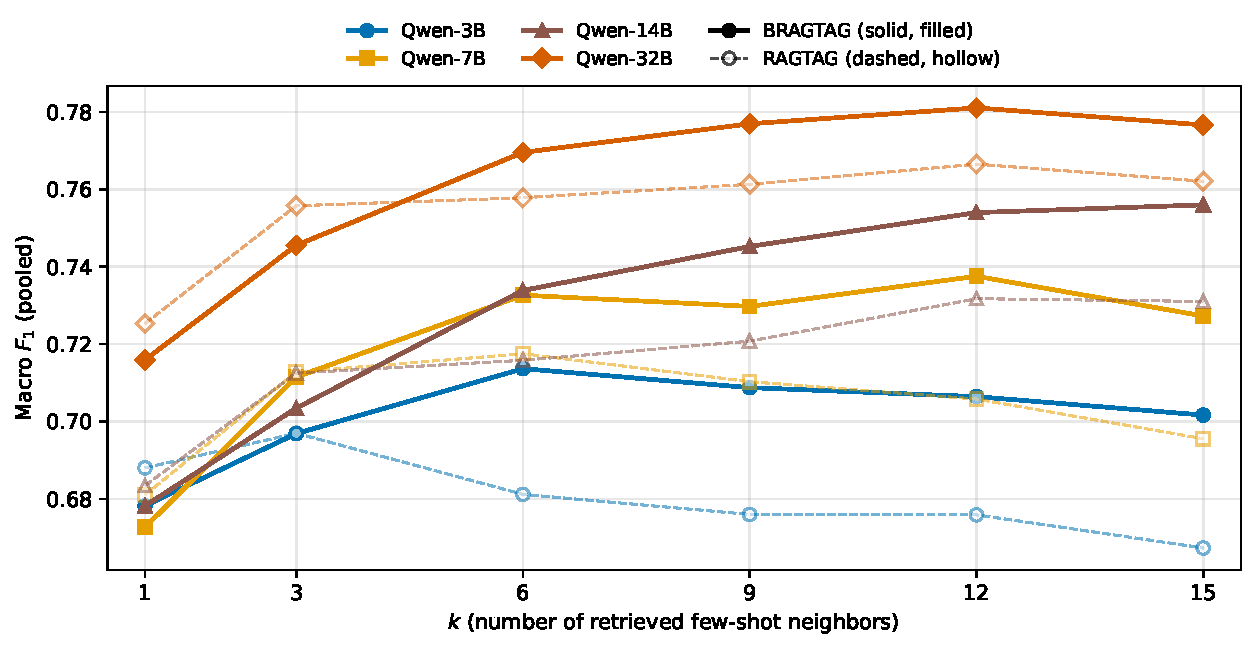
\includegraphics[width=0.7\linewidth]{figures/bragtag_kcurve.pdf}
    \caption{Macro $F_1$ as a function of $k$ across all model sizes for both \ragtag and \bragtag (project-specific setting)}
    \label{fig:bragtag-kcurve}
\end{figure}

Since the PS setting produced the best results for \ragtag, we use PS as the default for evaluating \bragtag\ on the same $k\in\{1, 3, 6, 9, 12, 15\}$ grid. \Cref{fig:bragtag-kcurve} shows macro F1 vs $k$ for both methods across all four model sizes. \bragtag\ outperforms \ragtag\ at every $k\ge 6$. At smaller $k\in\{1, 3\}$, \bragtag\ slightly underperforms by 0.001--0.010 macro F1, because the trigger fires too often and removes every retrieved example, practically reverting the query to zero-shot (40\% of queries at $k{=}1$ and 18\% at $k{=}3$).

% TODO (author): learn bootstrap CI methodology and re-audit the
% significance claim in this paragraph (CI numbers, footnote wording, and
% whether to add Wilcoxon/McNemar as supplementary tests). Stats produced
% by scripts/paper/significance_bragtag.py.
\bragtag's best $k$ almost always increases compared to \ragtag: Qwen-3B from $k{=}3$ to $k{=}6$, Qwen-7B from $k{=}6$ to $k{=}12$, Qwen-14B from $k{=}12$ to $k{=}15$, and Qwen-32B unchanged at $k{=}12$. When the trigger fires, \bragtag removes all bug examples from the top-$k$. Therefore, A higher initial $k$ is needed to leave enough remaining context for the LLM to use. At each method's best $k$, \bragtag\ outperforms \ragtag\ on every model. The paired bootstrap 95\% CI on the (\bragtag\ $-$ \ragtag) macro $F_1$ difference excludes zero in all four cells:\footnote{1{,}000 paired bootstrap resamples per model.} Qwen-3B $+0.017$ [+0.003, +0.031], Qwen-7B $+0.020$ [+0.007, +0.032], Qwen-14B $+0.024$ [+0.014, +0.034], and Qwen-32B $+0.014$ [+0.007, +0.022]. \Cref{tab:bragtag-results} reports the full best configuration comparison.

\begin{table}[t]
  \centering
  \caption{\ragtag\ vs \bragtag\ at each model's best $k$ (PS, pooled).}
  \label{tab:bragtag-results}
  \small
  \begin{tabular}{llccccccc}
    \toprule
    Model & Method & $k^*$ & Macro $F_1$ & $F_1^{\text{bug}}$ & $F_1^{\text{feat}}$ & $F_1^{\text{q}}$ & Invalid rate \\
    \midrule
    Qwen-3B & \ragtag & 3 & 0.697 & 0.711 & 0.803 & 0.577 & 0.2\% \\
     & \bragtag & 6 & 0.714 & 0.693 & 0.803 & 0.645 & 1.8\% \\
    \addlinespace[2pt]
    Qwen-7B & \ragtag & 6 & 0.718 & 0.731 & 0.816 & 0.605 & 3.5\% \\
     & \bragtag & 12 & 0.738 & 0.742 & 0.805 & 0.666 & 3.8\% \\
    \addlinespace[2pt]
    Qwen-14B & \ragtag & 12 & 0.732 & 0.735 & 0.838 & 0.622 & 4.5\% \\
     & \bragtag & 15 & 0.756 & 0.745 & 0.840 & 0.683 & 4.7\% \\
    \addlinespace[2pt]
    Qwen-32B & \ragtag & 12 & 0.767 & 0.759 & 0.842 & 0.699 & 4.6\% \\
     & \bragtag & 12 & 0.781 & 0.775 & 0.840 & 0.729 & 4.0\% \\
    \bottomrule
  \end{tabular}
\end{table}


\begin{figure}[t]
    \centering
    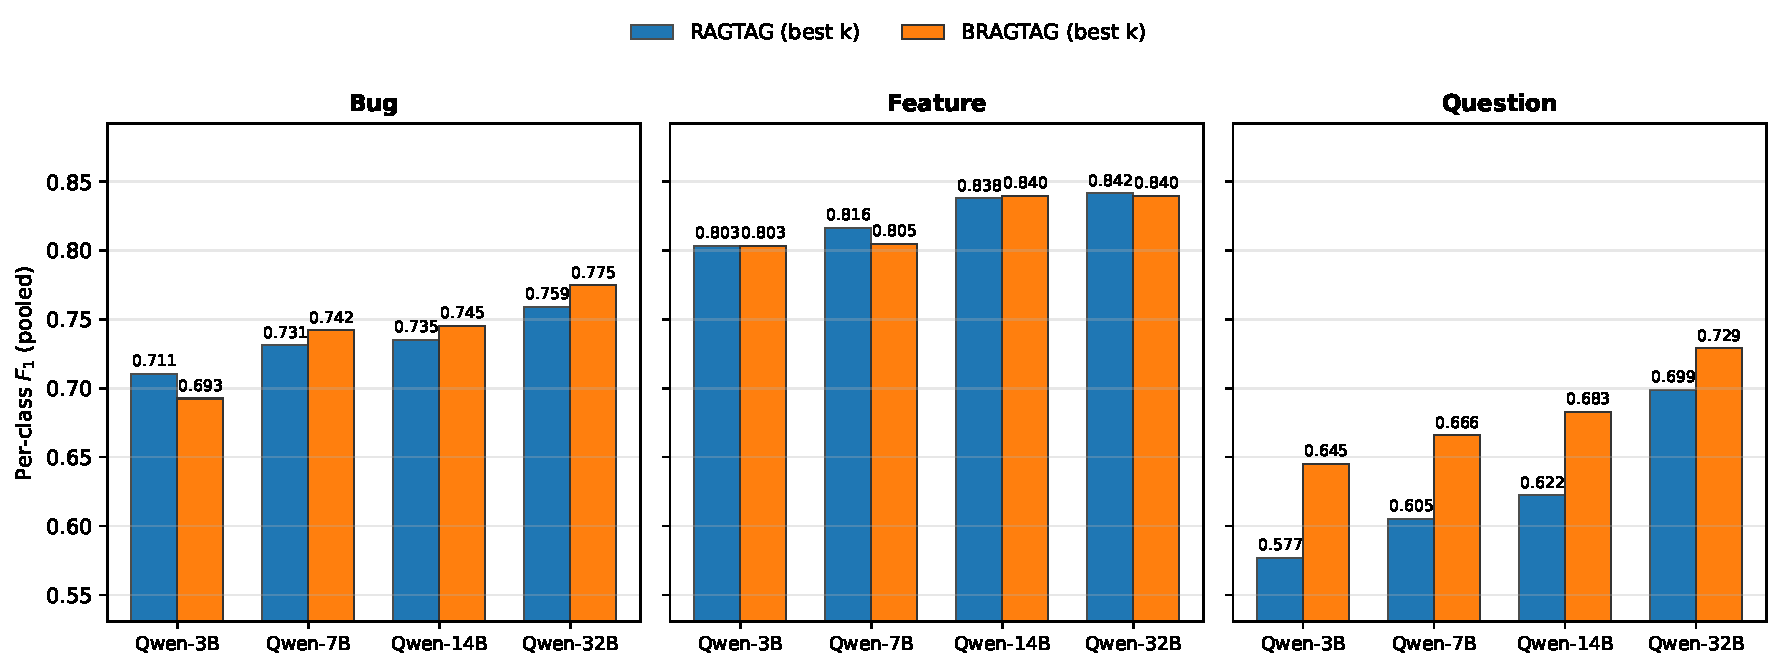
\includegraphics[width=\linewidth]{figures/bragtag_perclass.pdf}
    \caption{Per-class $F_1$ at each method's best $k$ across all model sizes for \ragtag\ and \bragtag.}
    \label{fig:bragtag-perclass}
\end{figure}

The performance gain comes from an increase on the question and bug classes with minimal impact on feature. \Cref{fig:bragtag-perclass} shows per-class $F_1$ at each method's best $k$. Question $F_1$ improves by 0.030--0.068 across all four model sizes. Bug $F_1$ stays within 0.018 of \ragtag, with a slight loss for Qwen-3B and slight gains for the larger models. Therefore, removing bug neighbors in some cases did not decrease overall bug performance. Feature $F_1$ is essentially unchanged. The question$\rightarrow$bug misclassification rate drops: at each model's best $k$, \ragtag\ misclassifies 26--36\% of true-question issues as bugs while \bragtag\ reduces this to 19--27\%. Averaged across $k\in[1,15]$, the rate drops from 31--40\% (\ragtag) to 24--36\% (\bragtag). Question$\rightarrow$feature misclassification is unaffected. This confirms that \bragtag's improvement comes from the targeted reduction of question$\rightarrow$bug misclassification.

Outputs from both approaches that failed to parse to a valid label are marked as \textit{invalid} and counted as incorrect. Averaged across $k\in[1,15]$, \bragtag\ has a lower invalid rate than \ragtag\ (2.3\% vs 3.0\% across the four models).


\subsection{RQ4. Can retrieval-augmented few-shot prompting match LoRA fine-tuning for IRC, and what are the costs of each approach?}
\label{sec:finetune-eval}
\label{sec:method-comparison}

\paragraph{Classification Performance.}

\begin{figure}[t]
    \centering
    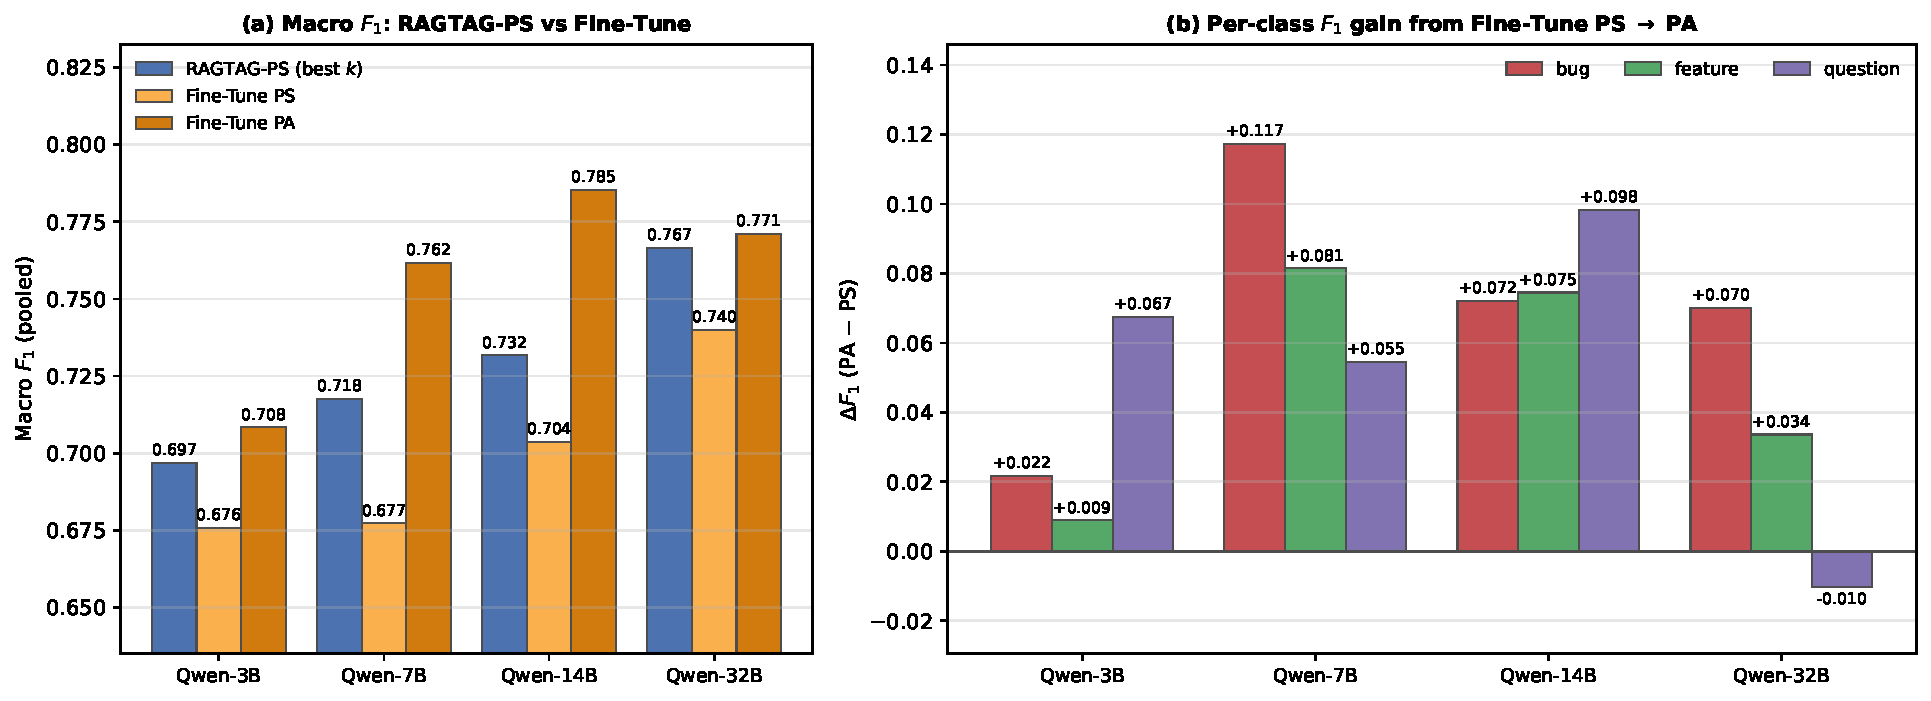
\includegraphics[width=\linewidth]{figures/finetune_comparison.pdf}
    \caption{\textbf{(a)} Macro $F_1$ for \ragtag at its best $k$ in PS vs Fine-Tune in PS and PA across all four model sizes. \textbf{(b)} Per-class $F_1$ gain from Fine-Tune PS to Fine-Tune PA ($\Delta F_1$ = PA $-$ PS) for each class and model size.}
    \label{fig:finetune-comparison}
\end{figure}

We fine-tune all models in both PA and PS settings. \Cref{fig:finetune-comparison}(a) compares macro $F_1$ for fine-tuning in both settings against \ragtag's PS at each model's best $k$. Fine-tune PA outperforms PS at every model size, by +0.033 (Qwen-3B), +0.084 (Qwen-7B), +0.082 (Qwen-14B), and +0.031 (Qwen-32B) macro $F_1$. This trend matches prior findings on LLM fine-tuning for IRC~\cite{heo2025study}.

\ragtag's PS outperforms Fine-Tune's PS at every model size, by +0.021 (Qwen-3B) to +0.040 (Qwen-7B) macro $F_1$. This shows that using only 300 labeled issues per project, retrieval-augmented few-shot is more effective than LoRA fine-tuning for IRC.

\Cref{fig:finetune-comparison}(b) shows where the additional PA training data helps most in fine-tuning. Averaged across all four models, bug $F_1$ gains +0.070 going from PS to PA, question gains +0.053, and feature gains +0.050. Qwen-32B is the only exception: its question $F_1$ drops by 0.010 while bug gains +0.070.

\begin{table}[t]
  \centering
  \caption{\ragtag, \bragtag, and Fine-Tune at each method's best configuration (\ragtag/\bragtag\ at their best $k$ on PS, Fine-Tune on PA). Macro $F_1$ and per-class $F_1$ are computed on raw predictions. The +\votag\ column reports macro $F_1$ with \votag as fallback for the invalid LLM outputs. Train and Inference are run-times on a single GPU with Total as their sum. RAM is the peak GPU memory observed}
  \label{tab:method-comparison}
  \footnotesize
  \setlength{\tabcolsep}{4pt}
  \resizebox{\linewidth}{!}{%
  \begin{tabular}{llcccccccccc}
    \toprule
    Model & Method & $k^*$ & Macro $F_1$ & +\votag & $F_1^{\text{bug}}$ & $F_1^{\text{feat}}$ & $F_1^{\text{q}}$ & RAM (GB) & Train (h) & Infer (h) & Total (h) \\
    \midrule
    Qwen-3B & \ragtag & 3 & 0.697 & 0.696 & 0.711 & 0.803 & 0.577 & 2.9 & -- & 0.18 & 0.18 \\
     & \bragtag & 6 & 0.714 & 0.720 & 0.693 & 0.803 & 0.645 & 2.9 & -- & 0.22 & 0.22 \\
     & Fine-Tune & -- & 0.708 & 0.711 & 0.736 & 0.790 & 0.599 & 5.5 & 0.31 & 0.11 & 0.42 \\
    \addlinespace[2pt]
    Qwen-7B & \ragtag & 6 & 0.718 & 0.729 & 0.731 & 0.816 & 0.605 & 6.8 & -- & 0.50 & 0.50 \\
     & \bragtag & 12 & 0.738 & 0.751 & 0.742 & 0.805 & 0.666 & 6.8 & -- & 0.60 & 0.60 \\
     & Fine-Tune & -- & 0.762 & 0.762 & 0.762 & 0.846 & 0.678 & 9.9 & 0.48 & 0.10 & 0.58 \\
    \addlinespace[2pt]
    Qwen-14B & \ragtag & 12 & 0.732 & 0.746 & 0.735 & 0.838 & 0.622 & 12.6 & -- & 1.37 & 1.37 \\
     & \bragtag & 15 & 0.756 & 0.771 & 0.745 & 0.840 & 0.683 & 12.6 & -- & 1.35 & 1.35 \\
     & Fine-Tune & -- & 0.785 & 0.785 & 0.792 & 0.828 & 0.736 & 16.7 & 1.49 & 0.22 & 1.71 \\
    \addlinespace[2pt]
    Qwen-32B & \ragtag & 12 & 0.767 & 0.779 & 0.759 & 0.842 & 0.699 & 22.3 & -- & 4.62 & 4.62 \\
     & \bragtag & 12 & 0.781 & 0.792 & 0.775 & 0.840 & 0.729 & 22.3 & -- & 4.15 & 4.15 \\
     & Fine-Tune & -- & 0.771 & 0.771 & 0.791 & 0.853 & 0.669 & 31.5 & 2.28 & 0.44 & 2.71 \\
    \bottomrule
  \end{tabular}%
  }
\end{table}


\Cref{tab:method-comparison} reports macro and per-class $F_1$ at each method's best configuration. \ragtag\ has competitive macro $F_1$ with fine-tuning: aggregated across the four model sizes (13{,}200 paired predictions), fine-tune leads \ragtag\ by 0.029 macro $F_1$ (paired bootstrap 95\% CI $[-0.037, -0.022]$). \ragtag\ is closer to fine-tune at the smallest and largest models and farther in the middle, with per-model (\ragtag\ $-$ fine-tune) macro $F_1$ deltas (paired bootstrap 95\% CIs in brackets) of $-0.011$ [$-0.028, +0.007$] (Qwen-3B), $-0.044$ [$-0.059, -0.029$] (Qwen-7B), $-0.053$ [$-0.068, -0.039$] (Qwen-14B), and $-0.004$ [$-0.020, +0.009$] (Qwen-32B). \ragtag\ and fine-tune are statistically equal at Qwen-3B and Qwen-32B.

\bragtag's balanced retrieval narrows this gap: the aggregate (\bragtag\ $-$ fine-tune) difference is $-0.010$ with paired bootstrap 95\% CI $[-0.018, -0.003]$, passing TOST equivalence at $\delta{=}0.02$.\footnote{1{,}000 paired bootstrap resamples per model for both \ragtag\ vs fine-tune and \bragtag\ vs fine-tune comparisons.} Similar to \ragtag, \bragtag\ performs better relative to fine-tune at the smallest and largest models: \bragtag\ is statistically tied with fine-tune at Qwen-3B and Qwen-32B while fine-tune leads on the mid-sized ones, with per-model (\bragtag\ $-$ fine-tune) deltas of $+0.006$ [$-0.012, +0.024$] (Qwen-3B), $-0.024$ [$-0.039, -0.009$] (Qwen-7B), $-0.029$ [$-0.044, -0.013$] (Qwen-14B), and $+0.010$ [$-0.005, +0.024$] (Qwen-32B).

\bragtag\ has the best question $F_1$ on Qwen-3B and Qwen-32B, while fine-tune leads on Qwen-7B and Qwen-14B. Fine-tune leads on bug across all four model sizes; on feature, \bragtag\ wins Qwen-3B and Qwen-14B while fine-tune wins Qwen-7B and Qwen-32B. These results show that \bragtag\ is able to compete with fine-tune due to its targeted question$\rightarrow$bug correction, boosting question $F_1$ without sacrificing bug or feature. Averaged across the four models, \bragtag\ is also the most class-balanced approach, with the lowest per-class $F_1$ standard deviation (0.058 vs 0.067 for fine-tune and 0.082 for \ragtag) and the highest worst-class $F_1$ floor (0.681 vs 0.671 and 0.626).

Fine-tune produces fewer invalid outputs than \ragtag\ and \bragtag\ in both settings, because the model learns the output format during training. Averaged across the four models, fine-tune's invalid rate is 0.28\% in PA and 0.38\% in PS, below \ragtag's 3.0\% and \bragtag's 2.3\% (averaged across $k\in[1,15]$). In an ideal triage scenario, every issue report receives a label, so a known limitation of LLMs is the production of outputs that do not comply with the instructions~\cite{sclar2023quantifying, akhavan2026linkanchorautonomousllmbasedagent}. To compensate for the invalid predictions we propose using \votag\ as a fallback mechanism. \votag\ never produces an invalid label and uses the neighbors already retrieved for \ragtag/\bragtag\ with no LLM inference cost. We apply the fallback to all three methods at their best data scopes for fair comparison: \votag-PS for \ragtag/\bragtag\ and \votag-PA for fine-tune. Under this protocol, \bragtag's reaches statistical equivalence with fine-tune, passing TOST at $\delta{=}0.01$ (bootstrap 95\% CI $[-0.007, +0.008]$).

\paragraph{Computation and Data Cost.}

\begin{figure}[t]
    \centering
    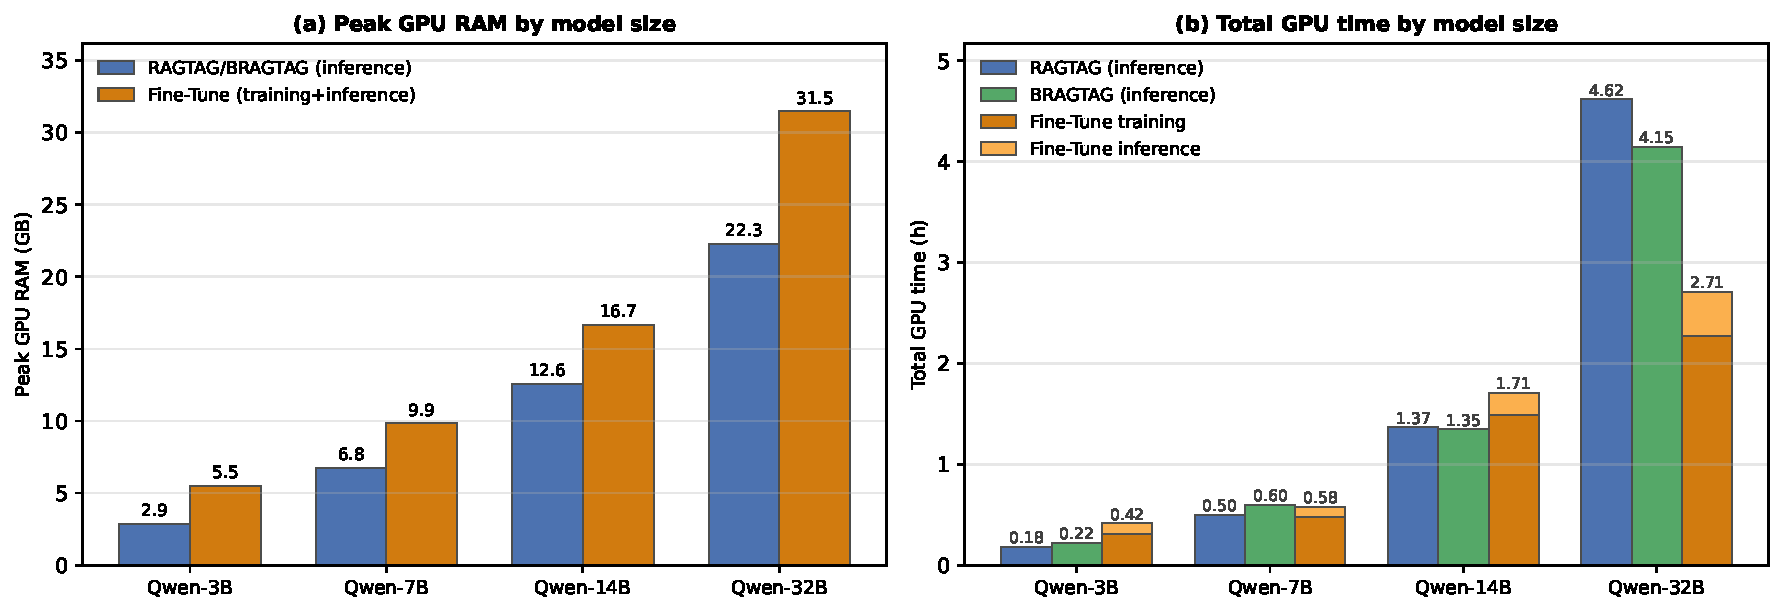
\includegraphics[width=\linewidth]{figures/cost_analysis.pdf}
    \caption{\textbf{(a)} Peak GPU RAM by model size: \ragtag/\bragtag inference vs Fine-Tune training + inference. \textbf{(b)} Total GPU time by model size: \ragtag\ and \bragtag\ vs Fine-Tune}
    \label{fig:cost-analysis}
\end{figure}

The methods have different hardware requirements. \Cref{fig:cost-analysis}(a) shows peak GPU RAM by model. \ragtag\ and \bragtag\ require identical GPU memory that grows with model size, while fine-tune requires more at every size due to training overheads such as, gradients, optimizer state, and activations retained for the backward pass. Averaged across the model sizes, \ragtag\ and \bragtag\ take 33\% less GPU memory than fine-tune (47\%, 31\%, 25\%, and 29\% less at Qwen-3B, 7B, 14B, and 32B respectively).


\Cref{fig:cost-analysis}(b) shows total GPU time at each model size. Fine-tune takes longer than \ragtag\ at Qwen-3B, 7B, and 14B. But at Qwen-32B fine-tune (2.71 h) takes less time than both \ragtag\ (4.62 h) and \bragtag\ (4.15 h). Inference time on each model naturally grows with prompt length. Fine-tune processes only the query issue, while \ragtag\ and \bragtag\ process significantly more context due to the additional few-shot examples per query. As a result, fine-tune inference takes much less time than rag-based inference, and fine-tune's total run-time is dominated by training. At Qwen-7B and Qwen-32B, \bragtag's inference cost alone exceeds fine-tune's combined training and inference time. \bragtag's intervention shortens the average context enough at Qwen-14B and Qwen-32B for \bragtag\ to run less than \ragtag. However, \bragtag runs longer at Qwen-3B and Qwen-7B because the intervention could not compensate for the higher best $k$ value.

Notably, \ragtag\ and \bragtag\ in PS retrieve only from 300 labeled issues per project, while fine-tune PA trains on the full 3{,}300 issues across all 11 projects to reach its best configuration. Therefore, at 11$\times$ less labeled data per project, \ragtag\ remains competitive with fine-tune, and \bragtag\ closes the gap to TOST equivalence at $\delta{=}0.02$, tightening to statistical equivalence at $\delta{=}0.01$ under the \votag\ fallback for invalid LLM outputs.




